% Jensen: zeros inside a circle, average of log|f| on the boundary.
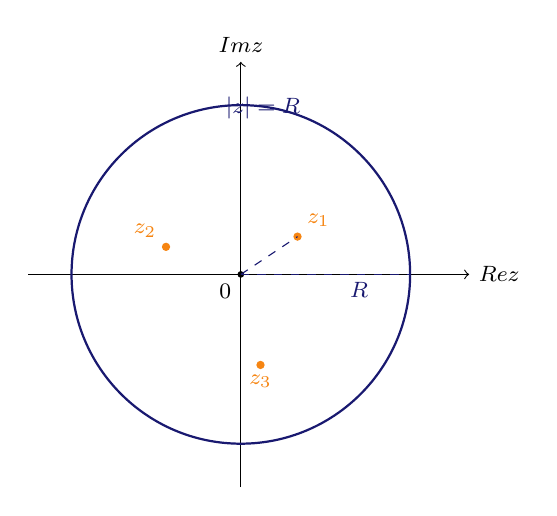
\begin{tikzpicture}[every node/.style={font=\footnotesize}]
  \draw[->] (-2.7,0)--(2.9,0) node[right] {$\operatorname{Re}z$};
  \draw[->] (0,-2.7)--(0,2.7) node[above] {$\operatorname{Im}z$};
  \draw[MidnightBlue,thick] (0,0) circle (2.15);
  \fill (0,0) circle (1.2pt) node[below left] {$0$};
  \fill[BurntOrange] (0.72,0.48) circle (1.5pt) node[above right] {$z_1$};
  \fill[BurntOrange] (-0.95,0.35) circle (1.5pt) node[above left] {$z_2$};
  \fill[BurntOrange] (0.25,-1.15) circle (1.5pt) node[below] {$z_3$};
  \draw[MidnightBlue,dashed] (0,0)--(0.72,0.48);
  \draw[MidnightBlue,dashed] (0,0)--(2.15,0);
  \node[MidnightBlue,below] at (1.5,0.02) {$R$};
  \node[MidnightBlue,above] at (0.28,1.85) {$|z|=R$};
\end{tikzpicture}
